\documentclass[11pt]{article}
\usepackage{xcolor}
\usepackage{pgfplots}
\usepackage[T1]{fontenc}
\usepackage[utf8]{inputenc}
\usepackage{xcolor}
\usepackage{pgfplots}
\usepackage{colortbl}
\usepackage{pgfplots}
\usepackage[T1]{fontenc}
\usepackage[utf8]{inputenc}
\usepackage{xcolor}

\begin{document}

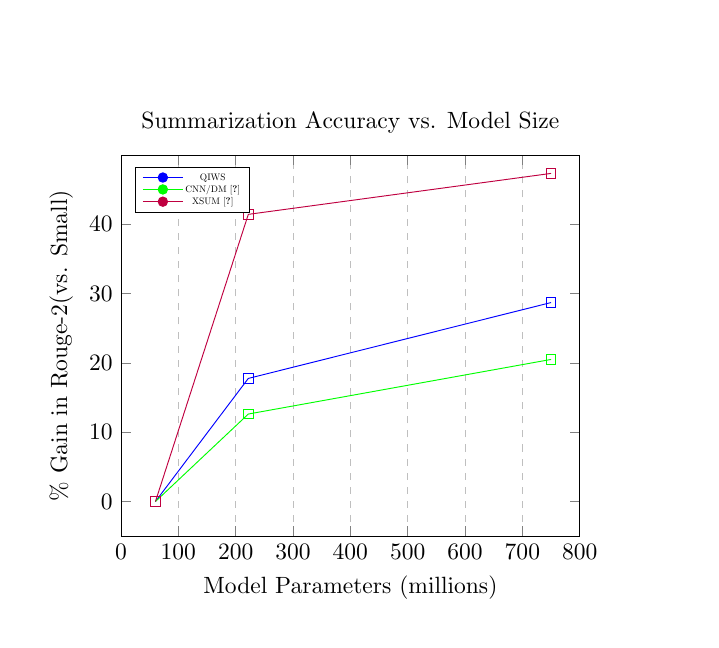
\begin{tikzpicture}
\scalebox{0.85}{
\begin{axis}[
    title={Summarization Accuracy vs. Model Size},
    ylabel={\% Gain in Rouge-2(vs. Small)},
    xlabel={Model Parameters (millions)},
    ymin=-5, ymax=50,
    xmin=0, xmax=800,
    ytick={0,10,20,30,40},
    xtick={0,100,200,300,400,500,600,700,800},
    legend pos=north west,
    xmajorgrids=true,
    grid style=dashed,
    legend style={nodes={scale=0.4, transform shape}}, 
    legend image post style={mark=*}
]
\addplot[
    color=blue,
    mark=square,
    ]
    coordinates {
    (60,0) ( 222,17.77) (750,28.72) 
    };
\addplot[
    color=green,
    mark=square,
    ]
    coordinates {
    (60, 0) (222, 12.63) (750,20.51)
    };  
\addplot[
    color=purple,
    mark=square,
    ]
    coordinates {
    (60,0) (222, 41.45) (750,47.36)
    };
\legend{QIWS, CNN/DM \cite{see-etal-2017-get}, XSUM \cite{Narayan2018DontGM} }
 \end{axis}}
\end{tikzpicture}

\end{document}